\begin{frame}
	\frametitle{geldfrei leben}
Eine Utopie für die meisten, aber eine Anregung zur Kreativität

{Alle sagten, das ist unmöglich. Da kam eine, die wusste das nicht und hat‘s einfach gemacht!}

	\begin{itemize}
		\item<1-> Perspektive Wechseln
		\item<2-> Eigene Grenzen testen
		\item<3-> Mit Entwurf an die Idee
		\item<4-> Machen statt Kaufen
	\end{itemize}
	\begin{center}
		\url{http://geldfreierleben.de/}
	\end{center}
\end{frame}
\note{Tobi Rosswog, Mitweltpädagoge schreibt ein e-Book um andere zu begeistern; utopival ein Festival ganz ohne Geld}

\begin{frame}
	\frametitle{Minimalismus}

	\begin{figure}
		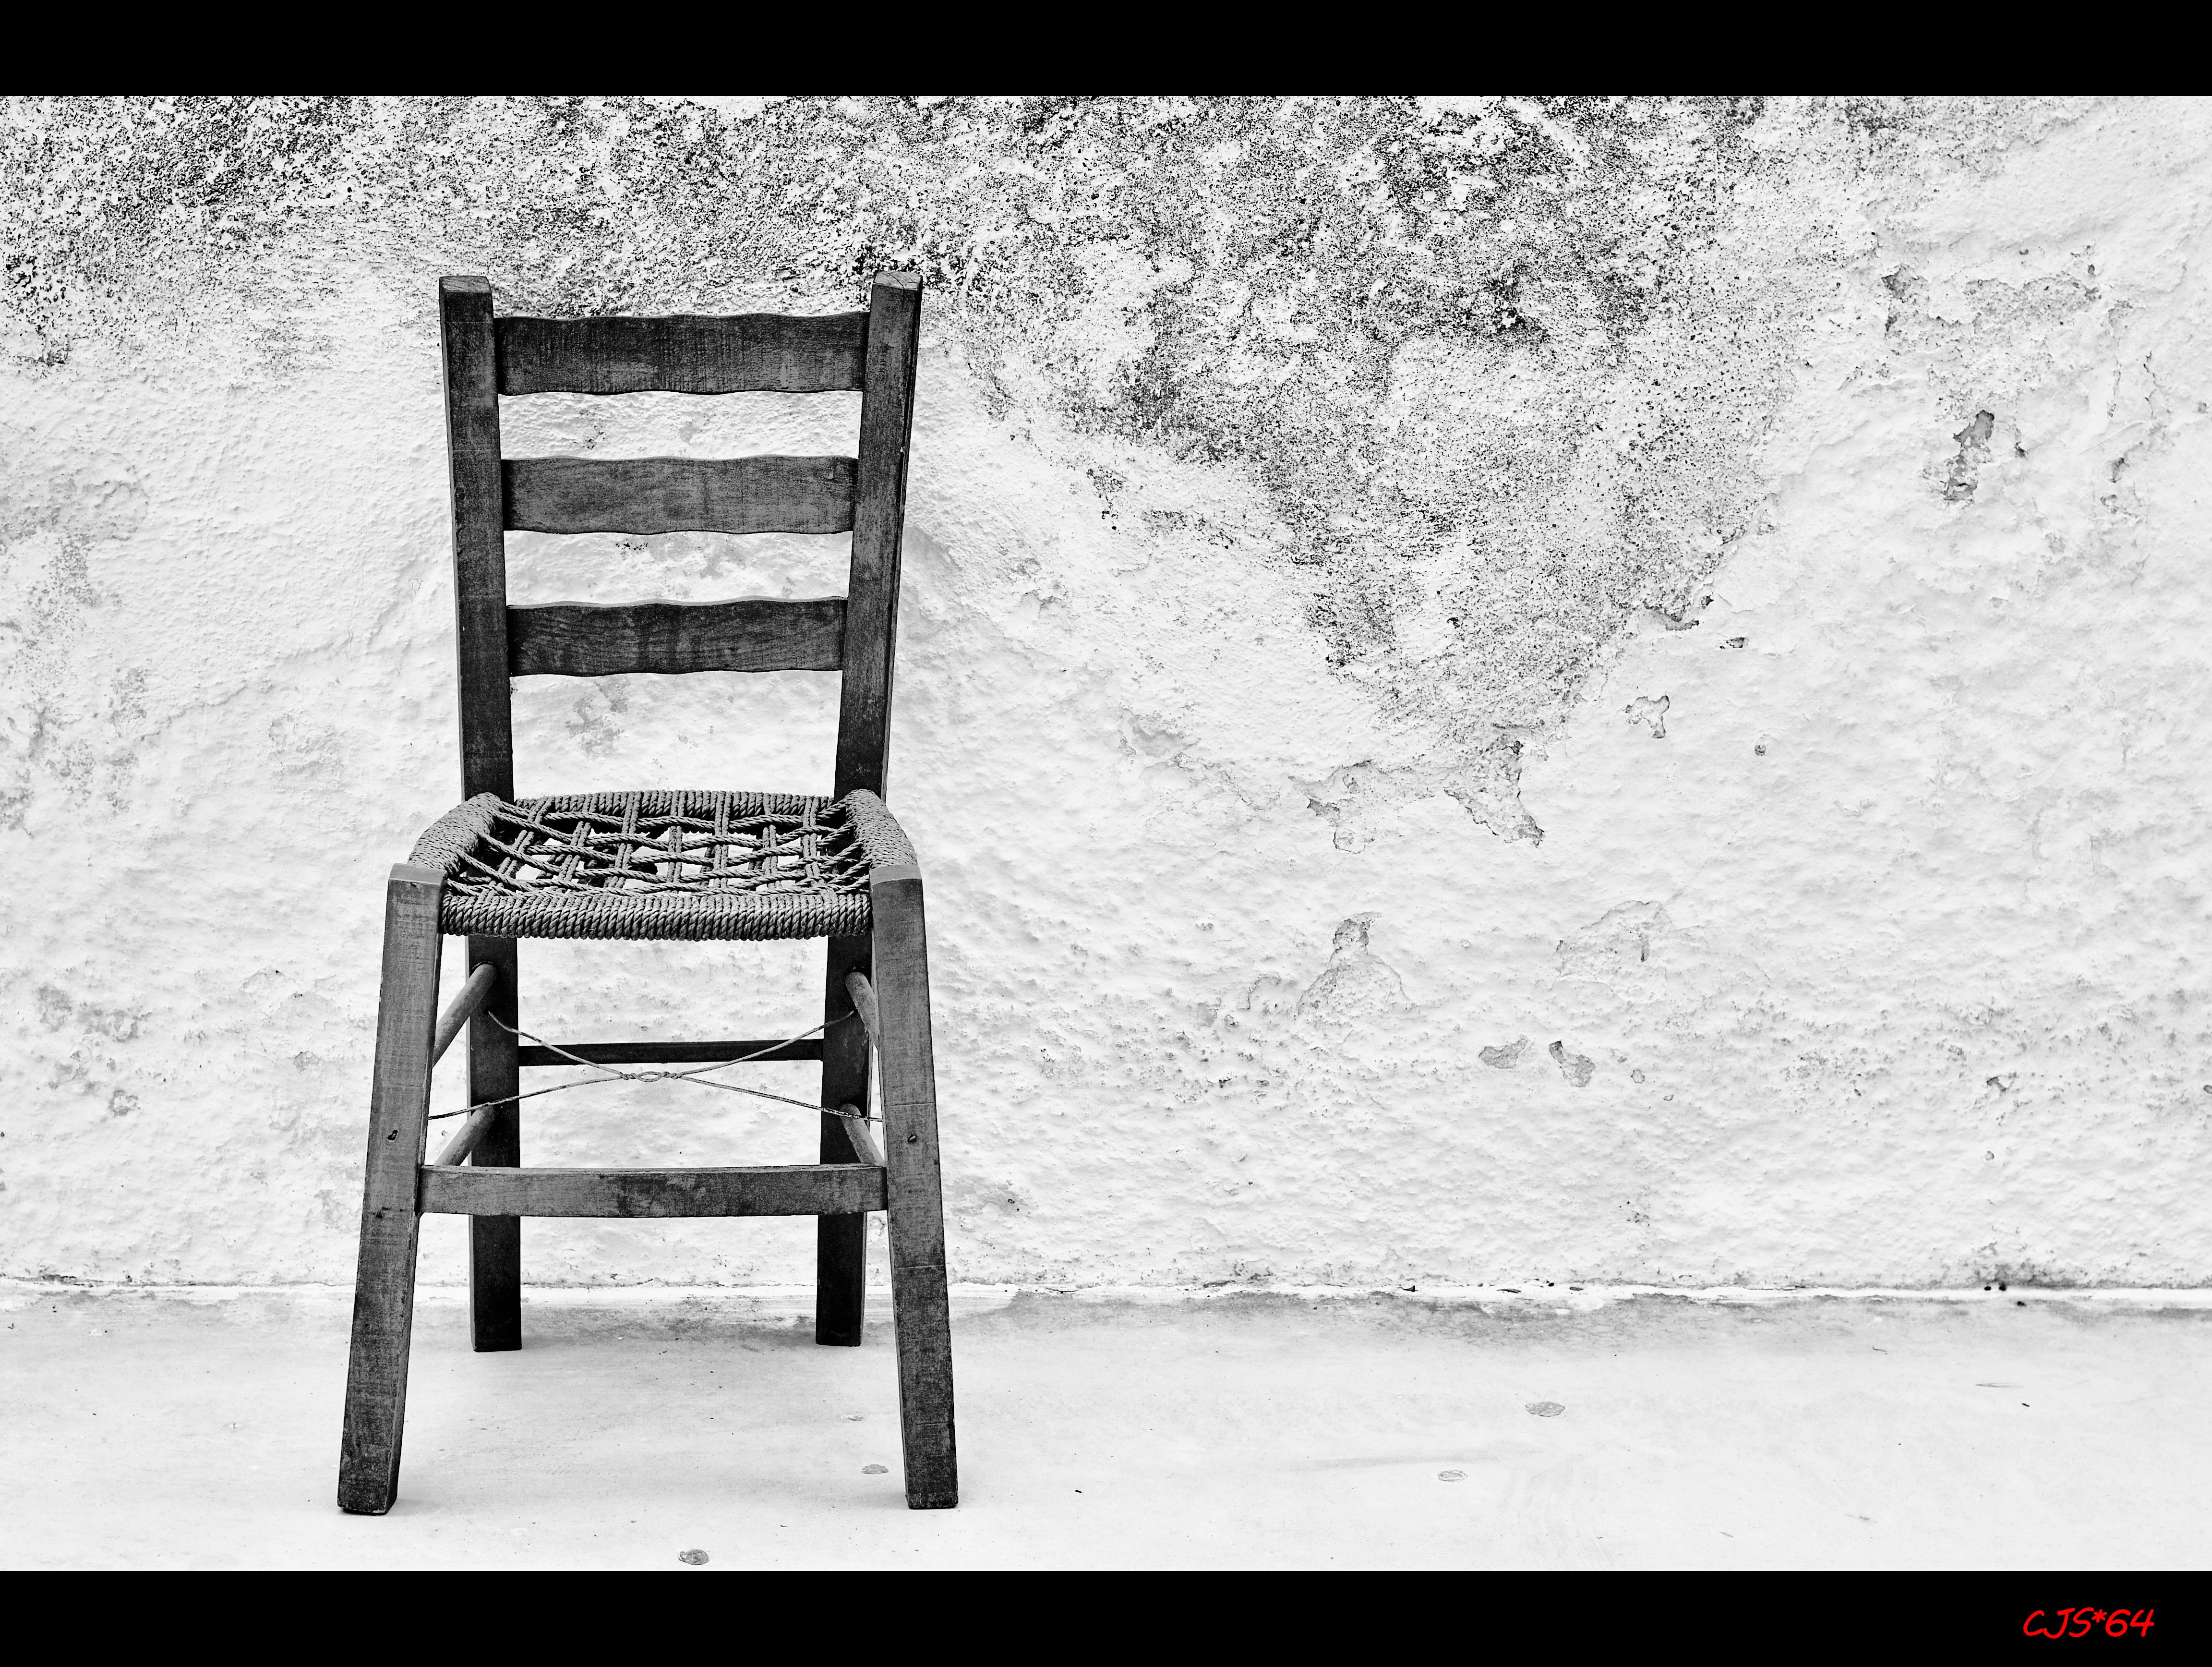
\includegraphics[height=0.7\textheight]{img/icecoldminimalism.jpg}
		\caption[Needs a cusion! by Craig Sunter]{\href{https://flic.kr/p/nT2jEf}{{Needs a cusion!}, Craig Sunter, CC BY-ND 2.0}}
	\end{figure}
\end{frame}
\note{
	$diameter$ 10.000 Gegenstände; 
	Verzicht auf Besitz;
	Maxmilmierung Lebensfreude;
	Reduktion < 1000 praktikabel
}

\begin{frame}
	\frametitle{Foodsharing}

	\begin{figure}
		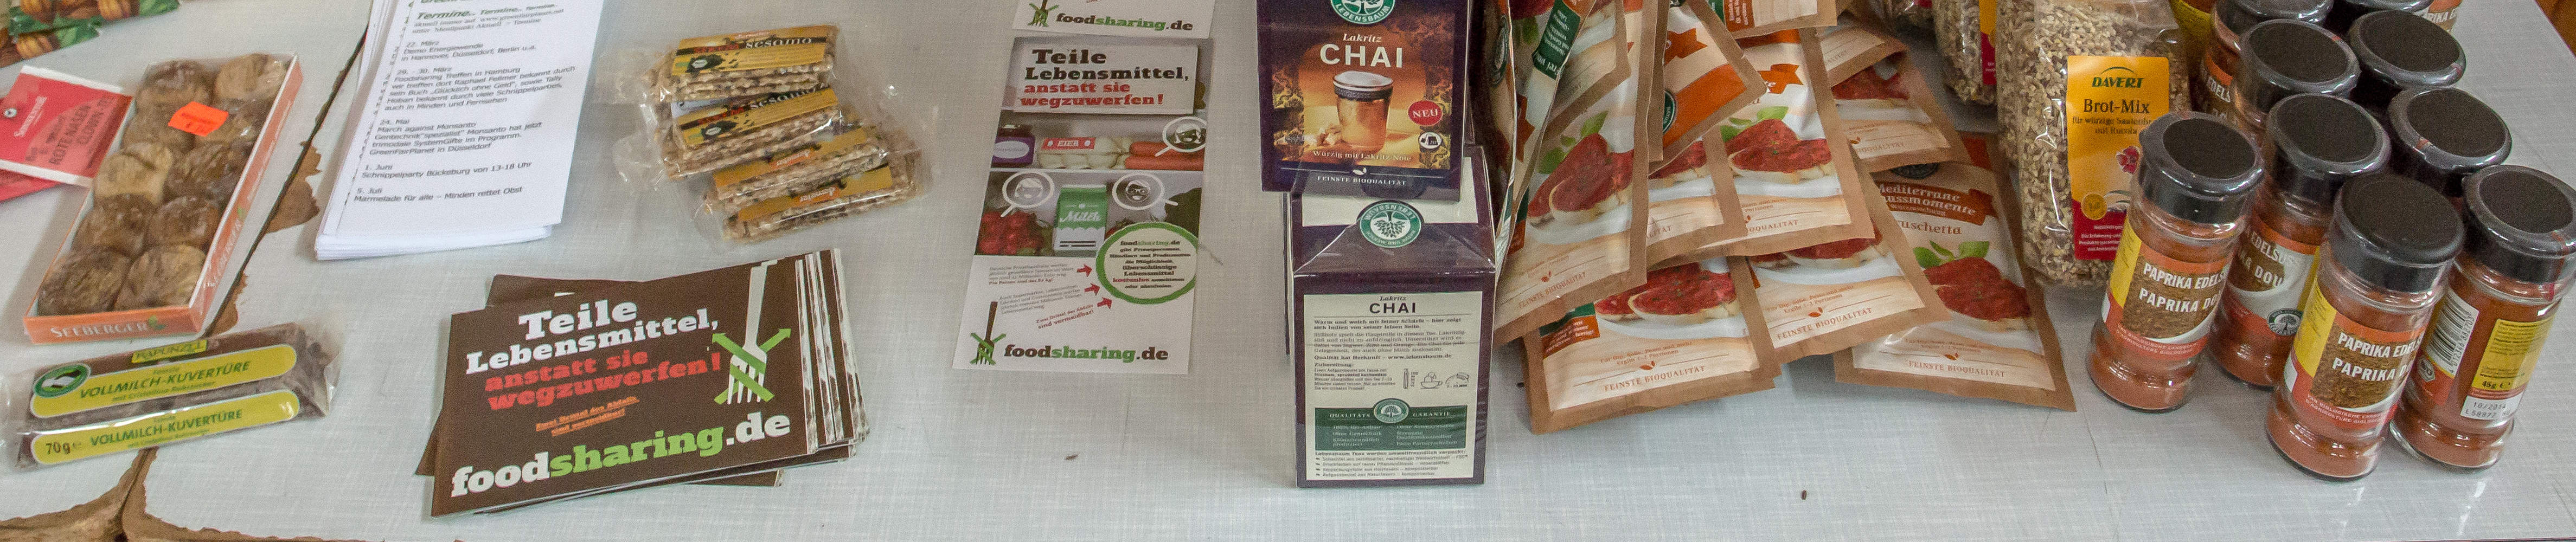
\includegraphics[width=0.9\textwidth]{img/foodsharing-cut.jpg}
		\caption[Foodsharing by Oliver Hallmann, Ausschnitt]{\href{https://flic.kr/p/kCmbVx}{{Foodsharing: Kochbar - Minden}, Oliver Hallmann, CC BY 2.0}}
	\end{figure}

	\href{https://foodsharing.de/}{Foodsharing}
\end{frame}
\note{Lebensmittel nicht wegwerfen, sondern teilen. Z.B. wenn Großabnahmen günstiger waren oder der Urlaub oder flexible Lebensführung den Konsum verhindern.}

\begin{frame}
	\frametitle{*Sharing}

	\begin{itemize}
		\item \href{http://mundraub.org/}{Mundraub}
		\item \href{https://www.kleiderkreisel.de/}{Kleiderkreisel}
		\item \href{http://www.hospitalityclub.org/}{Hospitality Club}, \href{http://couchsurfing.org/}{Couchsurfing}
		\item \href{http://c3jemx2ube5v5zpg.onion/}{Reading Club: Radical Militant Library} (via \href{https://www.torproject.org/}{Tor})
		%~ \item \href{https://bitcoin.org/de/}{Cryptocurrencies}
		\item \href{https://github.com/}{GitHub} – How people build software
		\item \href{https://freifunk.net//}{Freifunk} – WLAN-Gemeinschaftsnetze
	\end{itemize}
\end{frame}
\note{
Wo kann wann welche Frucht gepflückt werden; auch Rechtliche: Wo darf ich das?
Kleidertausch, kann gegen Geld oder andere Kleidung stattfinden; manche verschenken sogar was zuviel im Schrank ist
}
